\documentclass{article}
\usepackage{iclr2025_conference,times}
\usepackage{amsmath,amssymb}
\usepackage{booktabs}
\usepackage{graphicx}
\usepackage{url}
\usepackage{xcolor}
\usepackage[colorlinks=true,linkcolor=black,citecolor=black,urlcolor=blue!60!black]{hyperref}

\graphicspath{{../results/}}

\newcommand{\shrink}{\mathrm{shrink}}
\newcommand{\trcov}{\operatorname{tr}\mathrm{Cov}}
\newcommand{\E}{\mathbb{E}}
\newcommand{\Var}{\operatorname{Var}}
\newcommand{\arm}[1]{\texttt{#1}}

\iclrfinalcopy

\title{Shrinkage Baselines for GRPO on GSM8K:\\
When James--Stein Collapses, and What It Takes to Measure It}

\author{Hanwen Yang\\
\texttt{hanwenya150@gmail.com}\\
Code and logs: \url{https://github.com/hyang150/GRPO_JS_Eva}
}

\begin{document}
\maketitle

\begin{abstract}
GRPO estimates each prompt's baseline from the $N$ completions sampled for
that prompt alone; with small $N$ this mean is noisy. A given specification
proposes replacing it with a James--Stein estimator that shrinks each group
mean toward the batch mean, with the shrinkage constant fixed by assuming
unit per-sample reward variance. We implement the specification, five
alternative baselines behind one registry, and measure them on
Qwen2.5-0.5B-Instruct / GSM8K. Three results. (i)~Applied to raw $0/1$
rewards the specified estimator collapses onto the global batch mean: its
assumed variance overstates the true one by at least $4\times$, the collapse
is monotone in the number of prompts $K$, and at $N=2$ it is an algebraic
identity for every $K>6$. In three-seed training runs it discards the group
structure on 100\% of steps. (ii)~Establishing the specification's own
$\sigma^2\approx1$ precondition restores Stein's behaviour: the shrinkage
factor follows the closed form $N\tau^2/(1+N\tau^2)$ to within $0.02$, and
the baseline's mean squared error falls by 16--54\% in simulation.
(iii)~None of this is resolvable as end-to-end accuracy at this scale. The
two arms that are provably the same algorithm at $K=32,N=2$ finish $0.5$,
$6.5$ and $1.5$ points apart across seeds, against a literature effect of
$0.65$--$1.5$ points; the per-step gradient noise-to-signal ratio is 58--182
for every baseline alike. A paired gradient-variance measurement that an
earlier draft reported as significant is withdrawn after a projection bug
and an off-policy sampler were found, and was not repeated within the time
budget. We also show that the specification's optional division by the
within-group standard deviation multiplies degenerate-group advantages by
$10^4$ under any shrinkage baseline.
\end{abstract}

\section{Introduction}

Group Relative Policy Optimization~\citep{shao2024deepseekmath} removes the
critic from PPO~\citep{schulman2017ppo} by sampling $N$ completions per prompt
and using their mean reward as the baseline. With verifiable $0/1$ rewards
and small $N$ that baseline is a coarse estimate: at $N=2$ it takes three
values, and a group that is entirely right or entirely wrong carries no
signal at all. The specification this work was given (\texttt{GRPO.md},
reproduced in Appendix~\ref{app:spec}) proposes a remedy from classical
statistics: treat the $K$ group means in a batch as $K$ normal means with a
common known variance $V=1/N$ and shrink them toward the grand mean with the
positive-part James--Stein estimator~\citep{james1961}. Stein's result then
promises a lower total mean squared error, from which the specification
infers lower advantage variance, more stable training and support for
smaller $N$.

We set out to test that chain of inference end to end. The contributions
are:

\begin{itemize}\itemsep2pt
\item A registry of six baselines (Sec.~\ref{sec:estimators}) with a literal
      transcription of the specification asserted against the implementation
      to $10^{-12}$, an adapter to verl's advantage-estimator interface, and
      162 tests. The specification's own pseudocode is found to crash on two
      of the edge cases its prose claims to handle
      (Appendix~\ref{app:conformance}).
\item An analysis (Sec.~\ref{sec:analysis}) of when the specified estimator
      degenerates into the global mean: the large-$K$ limit of its shrinkage
      term, the $N=2$ identity, and the closed form the shrinkage factor
      follows once the precondition is honoured.
\item Simulation with known ground truth (Sec.~\ref{sec:synthetic}) and
      three-seed GRPO training at two group shapes with $K\cdot N=64$
      (Sec.~\ref{sec:training}), including a same-algorithm replicate pair
      that measures the protocol's noise floor directly.
\item A corrections record (Appendix~\ref{app:corrections}): an off-policy
      sampler, a completion-mask defect and a gradient-projection bug, all
      found in review, all fixed, and the withdrawal of the result they
      contaminated.
\end{itemize}

The headline is negative in two senses. The specification as written does
not work on $0/1$ rewards, and the corrected version, while it does what
Stein's theorem says it should to the baseline, produces no accuracy effect
that this scale of experiment can resolve.

\section{Background}

\paragraph{GRPO.} For prompt $x$ the policy samples $N$ completions
$y_1,\dots,y_N$ and receives rewards $r_i$. GRPO forms per-sample
advantages $A_i = r_i - b$ with $b$ the group mean, optionally divided by the
group standard deviation, and applies the PPO clipped surrogate with a KL
penalty toward a reference policy. Subtracting a baseline that does not
depend on the sample leaves the policy gradient unbiased and lowers its
variance; the group mean is a per-prompt Monte Carlo estimate of the value
function, which is what makes GRPO work without a critic. It is not
independent of $r_i$ --- it contains it --- but for the plain mean this only
scales the gradient by $(1-1/N)$; the leave-one-out mean of
RLOO~\citep{ahmadian2024rloo} removes even that.

\paragraph{The specification.} With group means $X_k=\frac1N\sum_i
r_i^{(k)}$, grand mean $\bar X$, $S=\sum_k(X_k-\bar X)^2$ and $c=V(K-3)$,
\begin{equation}
\tilde\mu_k=\bar X+\shrink\cdot(X_k-\bar X),\qquad
\shrink=\max\!\left(0,\;1-\frac{c}{S}\right),
\label{eq:js}
\end{equation}
and advantages are $A_i^{(k)}=r_i^{(k)}-\tilde\mu_k$. The specification sets
$V=1/N$, which is correct if the per-sample reward variance $\sigma^2$ is
$1$, and states in its theory section that rewards should first be rescaled
to make it so. Its pseudocode takes the raw reward matrix.

\section{Analysis}
\label{sec:analysis}

\subsection{The precondition, and what $K$ is}

On GSM8K the reward is binary, so $\sigma_k^2=p_k(1-p_k)\le\tfrac14$: at
least $4\times$ smaller than assumed, heteroscedastic across prompts, and
exactly zero for a group that is entirely right or entirely wrong (25--28\%
of groups at $N=8$ and 68--70\% at $N=2$ in our runs). Overstating $V$
overstates $c$, which drives $\shrink$ toward zero.

$K$ is the number of prompts whose rewards are on hand when advantages are
formed --- the rollout batch, not the backward micro-batch. Stein's
phenomenon needs $K\ge3$ for a fixed shrinkage centre and $K\ge4$ when the
centre is the estimated grand mean, hence $K-3$. This work runs $K=8$ and
$32$; \citet{zeng2025shrinking} run 64; production runs use hundreds to
thousands.

\subsection{The large-$K$ limit}

Since $\E[S]\approx(K-1)\Var(X_k)$ and $c=V(K-3)$, with $\tau^2$ the
variance of the true per-prompt pass rates,
\begin{equation}
\frac{c}{S}\;\xrightarrow[K\to\infty]{}\;
\frac{V_{\text{assumed}}}{\Var(X_k)}
=\frac{V_{\text{assumed}}}{\tau^2+\sigma^2/N},
\label{eq:limit}
\end{equation}
a constant. $K$ does not make the shrinkage stronger; it makes $S$ less
noisy, so the estimator converges to whatever this ratio says.

\textbf{If the precondition held}, $V_{\text{assumed}}=1/N$ is exact and
the limit is $1/(1+N\tau^2)<1$ for every $N$ and $\tau^2$: the clamp never
fires and
\begin{equation}
\shrink\;\xrightarrow[K\to\infty]{}\;\frac{N\tau^2}{1+N\tau^2},
\label{eq:eb}
\end{equation}
the empirical-Bayes posterior weight --- mild shrinkage that weakens as $N$
grows or as prompts spread apart.

\textbf{If it does not}, as for $0/1$ rewards, the ratio is at least
$(1/N)/(\tau^2+1/(4N))$. For the reward distribution used in
Sec.~\ref{sec:synthetic} it is $1.69$ at $N=8$ and $3.57$ at $N=2$. Above
$1$ the positive-part clamp fires and the estimator \emph{is} the global
mean. Larger $K$ makes this certain rather than occasional: the specified
method gets worse as the batch holds more prompts, which is the regime GRPO
is deployed in.

\subsection{The $N=2$ identity}
\label{sec:identity}

Group means of $0/1$ rewards lie in $[0,1]$, so $S\le K/4$ for any $K$. With
$c=(K-3)/N$ the clamp is guaranteed whenever $(K-3)/N>K/4$, i.e.\
$K>3/(1-N/4)$: $K>6$ at $N=2$, $K>12$ at $N=3$, and never guaranteed for
$N\ge4$, where it needs $S$ to be small, which Eq.~\eqref{eq:limit}
supplies as $K$ grows. At $N=2$, the regime the specification is motivated
by, the specified estimator therefore equals the global mean for every
batch of more than six prompts, independently of the rewards.
Sec.~\ref{sec:floor} turns this into a measurement.

\subsection{What does not transfer even under the precondition}

Three things. Bernoulli rewards are heteroscedastic, so a common known $V$
is an approximation established by pooling; the per-group standard
deviation cannot be used because it is zero for a third to two thirds of
groups. The shrunk baseline depends on $r_i$ itself through $\bar X$ and
$S$, so the policy gradient is biased --- not by the constant $(1-1/N)$
factor of plain GRPO but nonlinearly; only leave-one-out constructions keep
it unbiased. And a degenerate group receives a non-zero advantage by
design, which pushes all-correct prompts up and all-wrong prompts down in
whichever direction the batch happens to lean: noise traded for bias, not
signal created.

\subsection{The standard-deviation option}
\label{sec:footgun}

The specification offers ``divide by the within-group standard deviation
afterwards'' as an option. Under plain GRPO that is safe on a degenerate
group only because the advantage is exactly zero there, so
$0/(0+10^{-4})=0$. Every shrinkage baseline gives such a group a non-zero
advantage --- that is the point of the method --- so the same expression
multiplies it by $10^4$. Measured on GSM8K at $K=8$, $N=8$ with 38\%
degenerate groups: $\Var(A)=1.07\times10^5$ and gradient norm
$1.7\times10^3$; leaving zero-spread groups unscaled gives $0.57$ and
$1.2$. All experiments below use no standard-deviation scaling, which is
also the choice Dr.GRPO~\citep{liu2025drgrpo} argues for on other grounds.

\section{Estimators}
\label{sec:estimators}

\begin{table}[t]\centering\small
\begin{tabular}{llp{6.4cm}}
\toprule
name & baseline $b[k,i]$ & role \\
\midrule
\arm{vanilla}   & group mean                         & GRPO, the incumbent \\
\arm{rloo}      & leave-one-out group mean           & unbiased variance-reduction control \\
\arm{global}    & batch mean                         & \textbf{ablation}: what over-shrinkage degenerates to \\
\arm{js\_fixed} & Eq.~\eqref{eq:js}, $V=1/N$         & the specification as written \\
\arm{js\_pooled}& Eq.~\eqref{eq:js}, $V$ estimated   & the specification on $r/\sigma_{\text{pooled}}$, scaled back \\
\arm{js\_loo}   & two-level leave-one-out shrinkage  & \citet{zeng2025shrinking} \\
\bottomrule
\end{tabular}
\caption{Baselines. Without \arm{global} the comparison is uninterpretable:
``James--Stein helps'' cannot be told apart from ``any baseline other than
the group mean helps''.}
\label{tab:arms}
\end{table}

Table~\ref{tab:arms} lists the six. \arm{js\_pooled} is the
specification's ten steps applied after dividing the rewards by the pooled
within-group standard deviation $\sqrt{\operatorname{mean}_k s_k^2}$ and
scaling back; the identity is pinned by a test to $3\times10^{-16}$. We
read it as the specification with its own precondition honoured, not as a
different method. \arm{js\_loo} follows \citet{zeng2025shrinking},
Sec.~3.3, eq.~10 and 13--16, with both the group mean and the shrinkage
target leave-one-out. The registry mirrors verl's advantage-estimator
interface so any arm can be dropped into that framework through a thin
adapter. The training loop fixes everything that could confound a baseline
comparison: no KL term ($\beta=0$, no reference model), no
standard-deviation scaling, constant loss normalisation so completion
length does not reweight the update.

\section{Experiments}

\subsection{Simulation with known ground truth}
\label{sec:synthetic}

Ground truth is unavailable on GSM8K, so the baseline's error is measured
in simulation: $p_k\sim\mathrm{Beta}(1.2,2.2)$ (mean $0.35$, matching the
model's observed per-prompt spread; $\tau^2/\sigma^2=0.294$), rewards
$\sim\mathrm{Bernoulli}(p_k)$, 2000 trials at $K=32$ and 3000 at each $K$
of the sweep.

\begin{table}[t]\centering\small
\begin{tabular}{rrrrrrr}
\toprule
$N$ & degenerate & \arm{global} & \arm{js\_fixed} & \arm{js\_pooled} & \arm{js\_loo} & \arm{js\_pooled} $\shrink$ (Eq.~\ref{eq:eb}) \\
\midrule
2  & 64.5\% & $-39.6\%$  & $-39.6\%$  & $-54.4\%$ & $-51.3\%$ & 0.386 (0.370) \\
4  & 36.7\% & $+17.2\%$  & $+17.2\%$  & $-40.8\%$ & $-40.0\%$ & 0.547 (0.541) \\
8  & 18.7\% & $+131.1\%$ & $+131.0\%$ & $-26.7\%$ & $-27.0\%$ & 0.705 (0.702) \\
16 & 8.9\%  & $+355.5\%$ & $+258.8\%$ & $-15.8\%$ & $-16.0\%$ & 0.827 (0.825) \\
\bottomrule
\end{tabular}
\caption{MSE of the baseline against the true $p_k$ relative to
\arm{vanilla}, $K=32$. \arm{rloo} equals \arm{vanilla} exactly:
leave-one-out changes the baseline's independence, not its point estimate.
The last column gives \arm{js\_pooled}'s measured shrinkage factor with the
prediction of Eq.~\eqref{eq:eb} in parentheses.}
\label{tab:synth}
\end{table}

\begin{table}[t]\centering\small
\begin{tabular}{rrrrr}
\toprule
$K$ & \arm{js\_fixed} $\shrink$ & \arm{js\_fixed} MSE & \arm{global} MSE & \arm{js\_pooled} MSE \\
\midrule
4  & 0.333 & $+1.0\%$   & $+99.1\%$  & $-9.3\%$  \\
8  & 0.058 & $+84.3\%$  & $+116.4\%$ & $-18.7\%$ \\
16 & 0.006 & $+121.7\%$ & $+125.5\%$ & $-24.4\%$ \\
32 & 0.000 & $+130.2\%$ & $+130.5\%$ & $-26.8\%$ \\
64 & 0.000 & $+133.6\%$ & $+133.6\%$ & $-28.1\%$ \\
\bottomrule
\end{tabular}
\caption{Sweeping $K$ at $N=8$. By $K=64$ \arm{js\_fixed} and \arm{global}
agree to every digit. At $K=4$ the specified method is roughly neutral, so a
small-$K$ experiment would show nothing wrong.}
\label{tab:ksweep}
\end{table}

Table~\ref{tab:synth} gives the $N$ sweep. \arm{js\_fixed} is \arm{global}
for $N\le4$ and within $0.1\%$ of it at $N=8$: it discards the group
structure entirely, and for $N\ge4$ it is worse than plain GRPO. Estimating
$V$ fixes it, the gain growing as $N$ shrinks, which is the regime the
method claims; and the measured shrinkage follows Eq.~\eqref{eq:eb} to
within $0.02$. Table~\ref{tab:ksweep} shows the collapse deepening
monotonically in $K$, as Eq.~\eqref{eq:limit} predicts. Figure~\ref{fig:synth}
draws both.

\begin{figure}[t]\centering
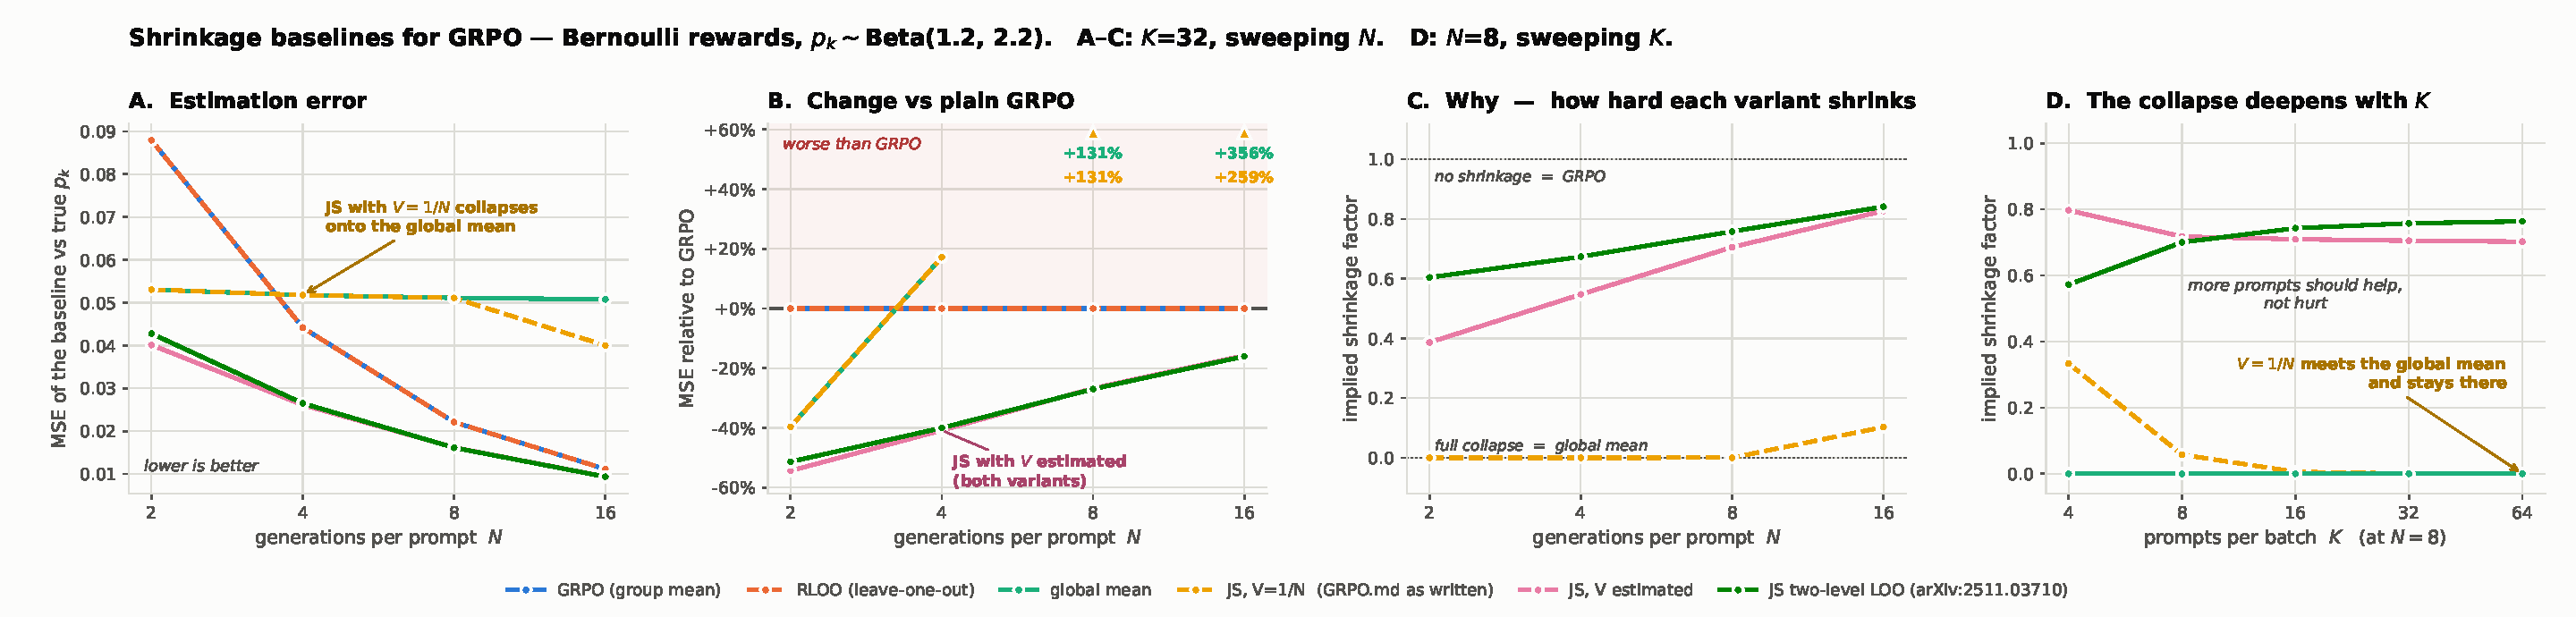
\includegraphics[width=\textwidth]{fig1_synthetic_mse.pdf}
\caption{A--C: sweeping $N$ at $K=32$; D: sweeping $K$ at $N=8$.
\arm{js\_fixed} (dashed) lies on \arm{global}; estimating $V$ recovers the
intended behaviour.}
\label{fig:synth}
\end{figure}

\subsection{GRPO on GSM8K}

Qwen2.5-0.5B-Instruct~\citep{qwen2025}, full fine-tune, GSM8K
\citep{cobbe2021gsm8k} with a rule-based correctness reward, 512 new
tokens, bf16 with gradient checkpointing, learning rate $10^{-6}$, PPO clip
$0.2$, one inner update per rollout. Development on one RTX~5080 (16\,GB;
11.0\,GiB peak, ${\sim}25$\,s per step at $K{=}8,N{=}8$), the three-seed
sweeps on two RTX~5090s. Every evaluation scores the same 200 test problems
greedily in the same order, so checkpoints are compared with McNemar's test
rather than by overlapping binomial intervals.

Two engineering points affect the numbers. Gradient checkpointing sets
\texttt{use\_cache=False}, which silently makes generation quadratic in
length; toggling it off around the rollout halved the step time. And pure
bf16 at $10^{-6}$ rounds most of the update away --- a weight of $0.0145$
has a ULP of $1.1\times10^{-4}$ while an AdamW step moves it by
${\sim}10^{-6}$; measured, $2.3\%$ of sampled weights change per step. The
fp32-master-weight recipe does not fit 16\,GB at this batch, so all arms
share the bf16 handicap.

\subsection{Three seeds, two group shapes}
\label{sec:training}

\begin{table}[t]\centering\small\setlength{\tabcolsep}{4pt}
\begin{tabular}{llrrrrrr}
\toprule
$K{\times}N$ & arm & final, per seed & mean $\pm$ sem & vs \arm{vanilla} & $p$ & $\shrink$ & collapsed \\
\midrule
$8{\times}8$  & \arm{vanilla}    & 44.5 / 42.0 / 47.5 & $44.7\pm1.6$ & & & 1.000 & 0 \\
$8{\times}8$  & \arm{js\_pooled} & 44.0 / 45.5 / 47.0 & $45.5\pm0.9$ & $+0.8\pm1.3$ & 0.60 & 0.85 & 0--1 \\
$8{\times}8$  & \arm{js\_fixed}  & 44.0 / 47.5 / 46.0 & $45.8\pm1.0$ & $+1.2\pm2.2$ & 0.65 & 0.21 & 38--44 \\
$8{\times}8$  & \arm{global}     & 48.5 / 44.0 / 45.0 & $45.8\pm1.4$ & $+1.2\pm1.9$ & 0.61 & 0.000 & 150 \\
\midrule
$32{\times}2$ & \arm{vanilla}    & 46.0 / 45.5 / 44.5 & $45.3\pm0.4$ & & & 1.000 & 0 \\
$32{\times}2$ & \arm{js\_pooled} & 41.0 / 46.0 / 47.5 & $44.8\pm2.0$ & $-0.5\pm2.4$ & 0.85 & 0.56 & 0--1 \\
$32{\times}2$ & \arm{js\_fixed}  & 43.5 / 42.0 / 41.5 & $42.3\pm0.6$ & $-3.0\pm0.3$ & 0.009 & 0.000 & 150 \\
$32{\times}2$ & \arm{global}     & 44.0 / 48.5 / 43.0 & $45.2\pm1.7$ & $-0.2\pm1.6$ & 0.93 & 0.000 & 150 \\
\bottomrule
\end{tabular}
\caption{Final test accuracy (200 problems, greedy) after 150 steps, seeds
0--2, corrected sampler. ``vs \arm{vanilla}'' is the within-seed paired
difference, $p$ a paired $t$-test with two degrees of freedom, $\shrink$
the run mean of the implied shrinkage factor, ``collapsed'' the number of
steps at exactly $0$ (range over seeds). Every run starts from the same
checkpoint, so accuracy at step~0 is 45.0\% for all 24.}
\label{tab:phase4b}
\end{table}

Four arms at each of two shapes with $K\cdot N=64$, so every arm sees the
same number of completions per step; every arm of a seed walks the same
prompt stream. Table~\ref{tab:phase4b} gives the result.

\paragraph{At $K=8$, $N=8$ nothing is resolved.} Every arm is within $1.2$
points of \arm{vanilla}, every sem exceeds the difference, every $p$ is
about $0.6$. The per-seed columns show why: the same arm moves 3--5 points
between seeds. Seed~0 alone would have said \arm{global} beats
\arm{vanilla} by $4.0$ points (McNemar $p=0.039$); seeds 1 and 2 put it at
$+2.0$ and $-2.5$.

\paragraph{At $K=32$, $N=2$ the one significant row is the noise floor.}
\label{sec:floor}
\arm{js\_fixed} at $-3.0\pm0.3$ ($p=0.009$) reads as a finding. But by
Sec.~\ref{sec:identity} it is \arm{global} at this shape: its logged
shrinkage is $0$ on all 150 steps of all three seeds, and its step-1 record
agrees with \arm{global}'s to the bit before the two processes diverge at
step~2, because sampled generation is not reproducible on GPU. The two arms
are therefore three same-seed replicates of one algorithm
(Table~\ref{tab:twins}): they end $0.5$, $6.5$ and $1.5$ points apart.
Pooling them as the six runs they are gives $-1.6\pm1.0$ against
\arm{vanilla} and the significance is gone. A $t$-test with two degrees of
freedom on three differences that happen to land within $0.5$ of each
other produces $p<0.01$ from nothing.

\begin{table}[t]\centering\small
\begin{tabular}{lrrr}
\toprule
seed & \arm{global} & \arm{js\_fixed} & difference \\
\midrule
0 & 44.0\% & 43.5\% & $+0.5$ \\
1 & 48.5\% & 42.0\% & $+6.5$ \\
2 & 43.0\% & 41.5\% & $+1.5$ \\
\bottomrule
\end{tabular}
\caption{The same algorithm run twice per seed ($K=32$, $N=2$). The spread
is the run-to-run term of this protocol. An earlier two-run estimate under
the 1.1 sampler was $3.0$ points.}
\label{tab:twins}
\end{table}

The effect reported for this setting is $0.65$--$1.5$ points
(\citet{zeng2025shrinking}, Table~2: JS minus GRPO at $N=8/4/2$ on this
model and task, $K=64$, 500 steps, five seeds). The noise floor is 2--5$\times$
the effect; resolving a one-point effect at this spread needs on the order
of 20--40 seeds per arm.

\paragraph{What the sweep does establish.} The specification verbatim, at
the $N=2$ it is motivated by, discards the group structure on 100\% of
steps (25--30\% at $N=8$); \arm{js\_pooled} keeps 56\% of it at $N=2$ and
85\% at $N=8$, the mild shrinkage Stein's result asks for. The ``more
stable training'' claim finds no support: no arm clipped a single gradient
step, sampled-token entropy fell from $0.52$ to $0.26$--$0.33$ for every arm
alike, and the per-step gradient noise-to-signal ratio
(\citet{zeng2025shrinking}, eq.~17--18, across micro-batches) is 58--182
with 32--45\% of steps returning a non-positive signal estimate. At 8 or 32
prompts per step the gradient is essentially all noise for every baseline,
and the ratio cannot separate them. Those steps are reported as
right-censored ($+\infty$) rather than dropped, which would bias the median
down. Figure~\ref{fig:train} shows seed~0 of both shapes.

\begin{figure}[t]\centering
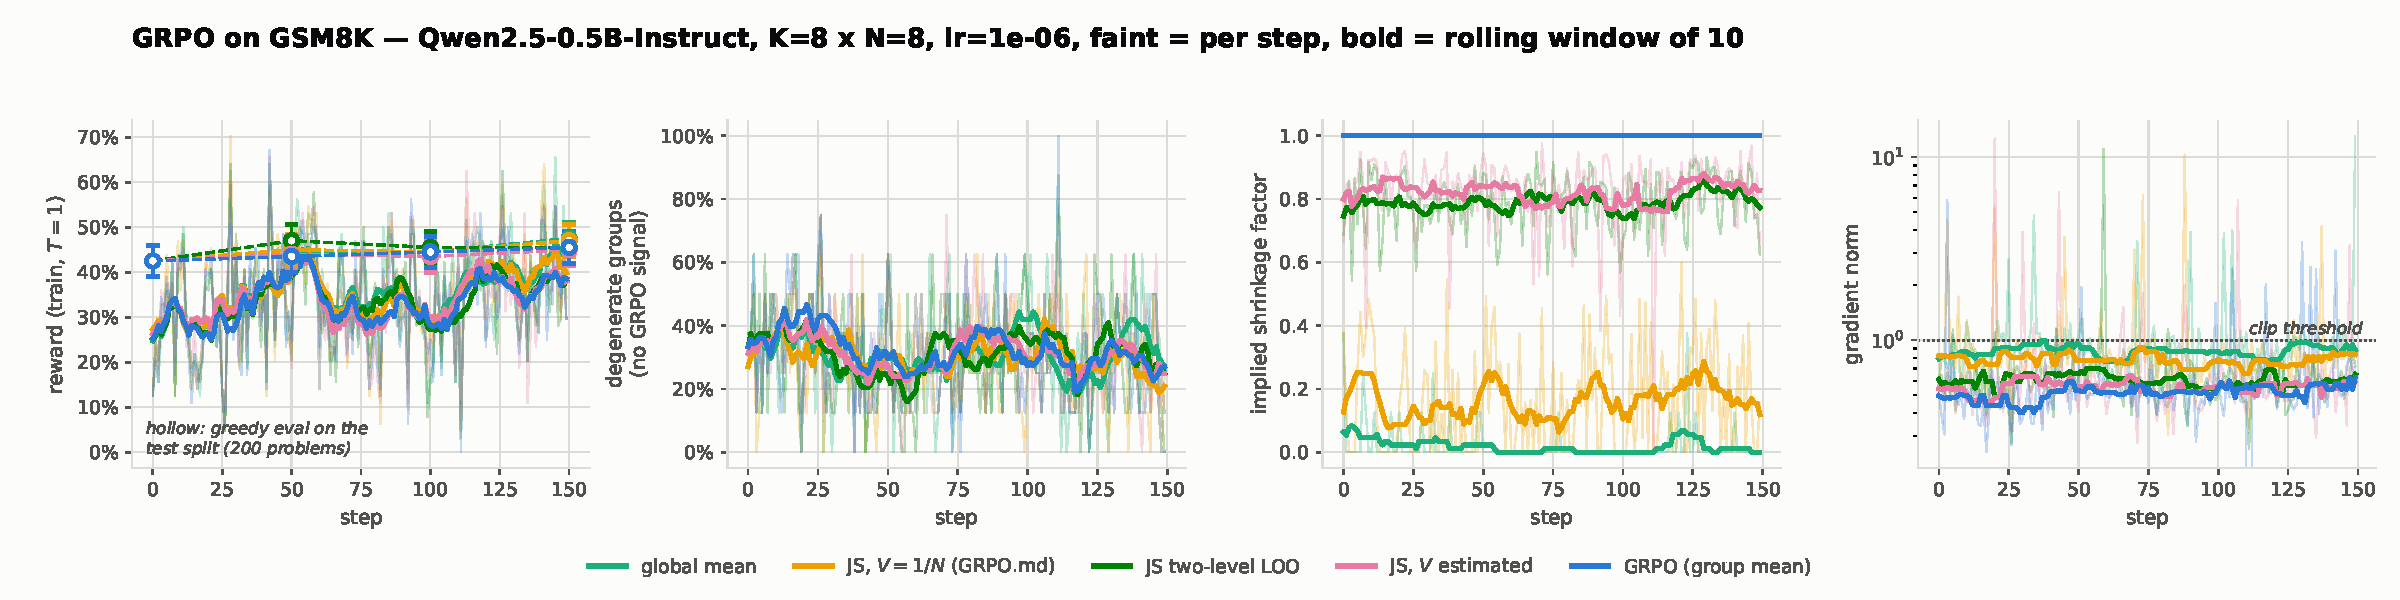
\includegraphics[width=\textwidth]{fig3_training.pdf}\\[4pt]
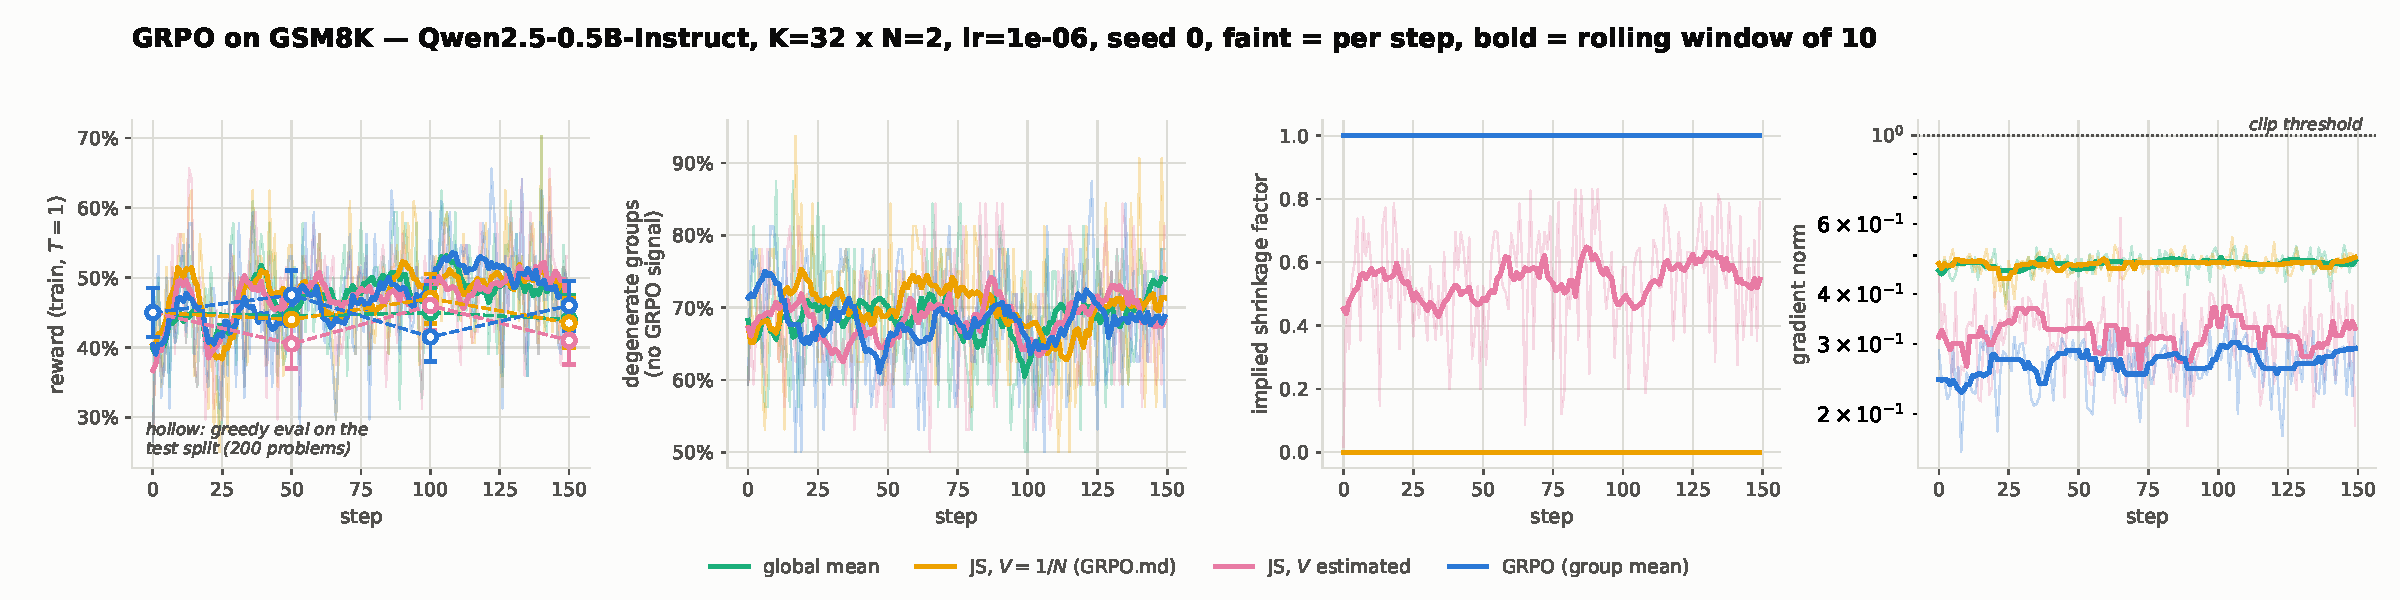
\includegraphics[width=\textwidth]{fig3_training_k32n2.pdf}
\caption{Seed 0 at $K{=}8,N{=}8$ (top) and $K{=}32,N{=}2$ (bottom). Reward
and degenerate-group panels overlap; the shrinkage panel separates the
arms, and at $N=2$ \arm{js\_fixed} lies on \arm{global}'s zero line for the
whole run. No gradient norm reaches the clip threshold.}
\label{fig:train}
\end{figure}

\subsection{A withdrawn measurement}
\label{sec:gradvar}

Because training runs cannot resolve the effect, an earlier draft measured
the estimator directly: every baseline scored the same frozen-policy
rollouts, and the trace of the gradient covariance over $\lVert\E[g]\rVert^2$
was estimated with Hutchinson probes and bootstrapped over 200 batches. It
reported \arm{js\_loo} at $-21.4\%$ $[-51.5,-7.8]$ against GRPO. Two
defects invalidate it: the probes reused random entries across equal-shaped
parameter tensors, and every rollout was drawn with the checkpoint's
default repetition penalty of $1.1$ rather than from the policy
(Appendix~\ref{app:corrections}). The instrument was also fragile on its
own terms, since $\lVert\E[g]\rVert^2$ was $8\%$ of $\E\lVert g\rVert^2$ and
obtained as a difference. The projection was fixed and a probe-free
estimator added --- for independent batches
$\E\langle g_b,g_{b'}\rangle=\lVert\E[g]\rVert^2$ exactly, so disjoint pairs
of batches give unbiased samples of both quantities --- and both are tested
on simulated gradients. The measurement was not repeated on the model
within the time budget. The historical table is in
Appendix~\ref{app:gradvar} as a record of the instrument, not as evidence.

\section{Related work}

\citet{zeng2025shrinking} is the same idea with its preconditions handled:
both the within-group and the between-prompt variance are estimated from
the batch, both levels are leave-one-out so the policy gradient stays
unbiased, and there are no hyper-parameters. That is \arm{js\_loo} here.
They report $0.65$--$1.5$ points over GRPO on this model and task at $K=64$
and $11$--$67\%$ lower gradient variance. EBPO~\citep{han2026ebpo} takes the
empirical-Bayes route: it shrinks toward a running global prior rather than
the batch mean, with shrinkage set by the within/between variance ratio.
Its stated feature --- an all-zero group still receives a non-zero signal
--- is the mechanism Sec.~\ref{sec:analysis} files under bias.
\citet{efron1975} applied James--Stein to binomial proportions, which is
exactly the $0/1$-reward case; their remedy for $\sigma^2\ne1$ was an
arcsine-square-root variance-stabilising transform before shrinking. We
pool the within-group standard deviation instead; the transform is the
more orthodox route and is untried here. RLOO~\citep{ahmadian2024rloo} and
Dr.GRPO~\citep{liu2025drgrpo} motivate the \arm{rloo} control and the
no-scaling default respectively.

\section{Limitations and conclusion}

Three seeds per arm at two group shapes leave every accuracy difference
inside its own standard error, and the same-algorithm pair spans $0.5$--$6.5$
points; no accuracy claim is made in either direction. The paired
gradient-variance measurement, the one instrument that could separate the
baselines at this scale, is withdrawn and was not repeated. \arm{rloo} and
\arm{js\_loo} were not included in the three-seed sweep. One model, one
task; whether the collapse threshold moves with reward density is untested.

What the work does establish is exact where it is exact. The specified
estimator, applied to $0/1$ rewards as its pseudocode does, is the global
batch mean --- asymptotically in $K$ for any $N$, and identically for every
$K>6$ at $N=2$ --- and the training logs show it. Honouring the
specification's own precondition restores the estimator Stein's theorem
describes, with a shrinkage factor that follows the empirical-Bayes closed
form. Whether that estimator improves training is a question this scale of
experiment cannot answer, and a protocol that reports a single seed, or a
$t$-test with two degrees of freedom, will answer it wrongly.

\bibliography{refs}
\bibliographystyle{iclr2025_conference}

\appendix

\section{The specification}
\label{app:spec}

\texttt{GRPO.md} gives, in order: the motivation (small-$N$ group means are
noisy); the model $X_k\sim\mathcal N(\mu_k,V)$ with $V=1/N$ under the
stated assumption that rewards have been rescaled so $\sigma^2\approx1$;
the positive-part James--Stein estimator of Eq.~\eqref{eq:js} with
$c=(K-3)/N$; ten implementation steps (group means, grand mean, $S$, $c$,
$K<4$ fallback, shrink factor with $\varepsilon$ guard, $S=0$ case, clamp,
shrunk means, advantages); a Python listing; and the optional division by
the within-group standard deviation.

\section{Conformance with the listing}
\label{app:conformance}

\texttt{tests/test\_spec\_conformance.py} transcribes the ten steps and,
separately, the Python listing character for character, and runs both
against the implementation. Away from the edge cases the listing and
\arm{js\_fixed} agree to $10^{-12}$ on continuous and on $0/1$ rewards. On
its own edge cases the listing does not run:

\begin{center}\small
\begin{tabular}{lp{8.6cm}}
\toprule
input & behaviour of the listing \\
\midrule
$K<4$ & \texttt{IndexError}: $\bar X$ is a 0-d tensor, so \texttt{unsqueeze(1)} is out of range \\
$S=0$ & \texttt{TypeError}: Python's \texttt{max(S, eps)} returns the float \texttt{eps} once $S<\varepsilon$, and \texttt{torch.clamp} rejects a float \\
$K=8$, $N=8$, $0/1$ rewards, $S>0$ & runs, and equals \arm{js\_fixed} \\
\bottomrule
\end{tabular}
\end{center}

Two departures, both asserted. Step~5's prose returns the per-group means
for $K<4$; the listing, once its indexing is repaired, returns rewards
centred on the global mean --- the \arm{global} arm, no longer GRPO. We
follow the prose. Step~7's ``$S=0\Rightarrow$ shrink factor $1$'' is
unreachable in the listing; we clamp to $0$ instead, which is
observationally identical since $S=0$ forces $\mathrm{diff}=0$.

\section{Corrections}
\label{app:corrections}

Found in review after the first draft; all fixed in code.
\begin{enumerate}\itemsep2pt
\item \textbf{Off-policy rollouts (2026-09-04).} \texttt{generate()} set
      temperature, top-$p$ and top-$k$ but not
      \texttt{repetition\_penalty}, which fell through to the checkpoint's
      \texttt{generation\_config} --- $1.1$ for Qwen2.5-Instruct.
      Completions were sampled from a penalised distribution while the loss
      used the raw policy's log-probabilities, in every arm of every
      experiment. The loop now passes $1.0$ explicitly. The three-seed
      sweeps of Sec.~\ref{sec:training} were run after this fix; the
      seed-0 five-arm sweep of Appendix~\ref{app:seed0} and the gradient
      measurement were not.
\item \textbf{Projection bug (2026-09-03).} The Hutchinson probes reused
      random entries across equal-shaped parameter tensors. Fixed
      (continuous stream per probe); regression tests compare projected
      with exact covariance.
\item \textbf{Completion mask (2026-09-04).} Only \texttt{<|im\_end|>}
      counted as a stop token; Qwen2.5 also stops on
      \texttt{<|endoftext|>}, which is its pad token, so such a completion
      was scored as 512 valid tokens including padding. The mask now stops
      on every terminator plus the pad id.
\item \textbf{Shrinkage diagnostic (2026-09-04).} Groups whose mean equals
      the grand mean were logged as unshrunk rather than undefined. The
      synthetic tables were regenerated with the corrected diagnostic
      (\arm{global} now reads its definitional $0$; MSE columns moved by
      under $1.5$ points).
\end{enumerate}

\section{Seed-0 sweep under the 1.1 sampler}
\label{app:seed0}

The first sweep, superseded, kept for the record: five arms, 150 steps,
same seed, same 200 test problems.

\begin{center}\small
\begin{tabular}{lrrrrrr}
\toprule
arm & eval@0 & eval@final & $\Delta$ & $p$ & $\shrink$ & collapsed \\
\midrule
\arm{vanilla}    & 42.5\% & 45.5\% & $+3.0$ & 0.24 & 1.000 & 0/150 \\
\arm{js\_pooled} & 42.5\% & 45.0\% & $+2.5$ & 0.27 & 0.850 & 1/150 \\
\arm{js\_loo}    & 42.5\% & 45.5\% & $+3.0$ & 0.21 & 0.818 & 0/150 \\
\arm{js\_fixed}  & 42.5\% & 47.0\% & $+4.5$ & 0.11 & 0.202 & 64/150 \\
\arm{global}     & 42.5\% & 47.5\% & $+5.0$ & 0.06 & 0.025 & 133/150 \\
\bottomrule
\end{tabular}
\end{center}

Nothing is significant; the 2.5-point spread across five arms is below the
floor one arm shows against itself. The shrinkage column separates into
tiers accuracy cannot resolve, and \arm{js\_pooled} and \arm{js\_loo},
derived independently, land within $0.03$ of each other. \arm{global}'s
$0.025$ is the diagnostic artefact of Appendix~\ref{app:corrections}. This
sweep's clip counts (36 of 150 steps for \arm{global} against 9 for
\arm{vanilla}) and entropy differences vanish under the corrected sampler.

\section{The withdrawn gradient measurement}
\label{app:gradvar}

200 paired batches, $K=8\times N=8$, policy frozen, mean accuracy 29.1\%,
1.1 sampler, buggy projection. Intervals were a paired bootstrap over
batches conditional on 24 probes.

\begin{center}\small
\begin{tabular}{lrrl}
\toprule
baseline & noise/signal & vs GRPO & \\
\midrule
\arm{vanilla}    & 11.5 & ---                      & \\
\arm{rloo}       & 11.5 & $-0.3\%$ $[-2.5,+6.9]$   & instrument check \\
\arm{js\_loo}    & 9.1  & $-21.4\%$ $[-51.5,-7.8]$ & withdrawn \\
\arm{js\_pooled} & 9.9  & $-14.4\%$ $[-38.2,+0.8]$ & withdrawn \\
\arm{js\_fixed}  & 6.0  & $-48.1\%$ $[-81.3,-15.8]$& biased estimator \\
\arm{global}     & 5.8  & $-49.7\%$ $[-83.5,-15.6]$& biased estimator \\
\bottomrule
\end{tabular}
\end{center}

Even had the numbers stood, \arm{js\_fixed} and \arm{global} would not be
``best'': they target a different $\E[g]$, since handing an all-correct
group a positive advantage inflates $\lVert\E[g]\rVert^2$ with a component
that merely pushes up easy prompts. A larger denominator is not more
signal.

\section{Reproduction}

\begin{verbatim}
uv sync && python main.py smoke
python -m pytest tests/ -q          # 162 tests
python main.py synthetic --k 32 --n 2 4 8 16
python experiments/synthetic_mse.py --k 4 8 16 32 64 --n 8 \
    --trials 3000 --out results/synthetic_k_sweep.json
python main.py sweep --seeds 0 1 2 --k 32 --n 2 --track-grad-var \
    --baselines vanilla js_fixed js_pooled global
python main.py sweep --seeds 0 1 2 --k 8  --n 8 --track-grad-var \
    --baselines vanilla js_fixed js_pooled global
python main.py compare --glob 'train_*_k8n8_s*.jsonl'
python main.py compare --glob 'train_*_k32n2_s*.jsonl'
python main.py figures
\end{verbatim}

The 24 per-step logs of Sec.~\ref{sec:training} are committed under
\texttt{results/}; they are not reproducible bit-for-bit
(Sec.~\ref{sec:floor}), which is why they are kept.

\end{document}
